\section{Introduction}

The field of bioinformatics exists at the intersection of biological research and computer science. The three key facets of the discipline are:

\begin{enumerate}
\item The creation and management of large scale datasets
\item The design of algorithms and statistical techniques aimed at teasing out relationships between members of those datasets
\item The use of these tools to improve medical science, whether it be drug discovery, tailoring treatments to individuals, or identifying trends in public health.
\end{enumerate}

Much of bioinformatics revolves around genetic information. The potency of genetic data lies partially in its ability to uniquely identify an individual and provide information on various social groupings that individual is a member of, whether it be family, disease group, or ethnic group. This property allows an individual's genetic data to be predictive of not only their health, but the health of others. The analysis of genetic data thus has tremendous potency, both to help others and to compromise privacy. This Systematization of Knowledge paper aims to summarize the state of the subset of bioinformatics concerned with ensuring both the privacy of individuals.

\section{Secure Multiparty Computation}

A de facto requirement to providing adequate privacy for bioinformatics applications is secure computation. In secure computation, there are two or more parties who each have some private data, and it is necessary to answer a question that relies on everyone's data. For example, in a vote, the majority winner must be identified. In an auction, the winning bid must be identified. Simultaneously, however, each party wants to maximize their privacy, i.e. each voter doesn't want who they voted for to be revealed.

\paragraph{Formal Definition}
There are $n$ parties, where $x_i$ is the private input of the $i$th party, and there is a function $f(x_1, x_2, ..., x_n)$ that everyone wishes to compute. 

For the two party case, it can be shown that the output of $f$ can be determined without leaking any information about the private inputs for any arbitrary function $f$.

The two parties are traditionally named Alice and Bob, where Alice will have secret information $a$, Bob will have secret information $b$, and the function $f$ is a public function whose output Alice and Bob both want to know without revealing additional information about $a$ or $b$ respectively. As an example, Alice and Bob have both just received their MCAT scores, and want to know who scored higher on the exam without revealing their exact scores. Here, $a$ is Alice's score, while $b$ is Bob's score. The function $f$ they wish to securely compute is:  

\begin{equation}
f(a,b)= \begin{cases}
Alice, & \text{if $a > b$}.\\
Bob, & \text{if $b < a$}.\\
same, & \text{otherwise}.
\end{cases}
\end{equation}

\paragraph{Security Guarantee}
In our imagined scenario, both Alice and Bob will adhere to the \textit{Honest-but-Curious} model. In this model, neither Alice or Bob will lie, and both will follow the protocol. However, both Alice and Bob will analyze any messages sent between them and try to identify the other person's input.

\paragraph{}
It is important to note that the assumption that Alice and Bob will not lie is a fairly tenuous one. It is still fairly difficult to build a secure protocol even in this relaxed scenario, and the Honest-but-Curious threat model is often used as stepping stone towards a stronger protocol. This paper shall ignore the existence of malicious adversaries as it relates to secure computation.

\paragraph{Ideal World Scenario}
In order to evaluate the eventual solution, we will compare it to the best case scenario. In this ideal scenario, Alice and Bob would each hand their private data to a trusted third party, Faith. Faith would compute $f(a,b)$ and return the output to Alice and Bob without revealing either input.

Even this ideal scenario can leak information. To see this, consider $f(a, b) = a + b$. Knowing the output, both Alice and Bob can determine the other's private data. Any proposed solution must therefore not leak very much more information than what can be learned with your own private data and the output of $f$. 

\paragraph{Encryption}
A concept that will be important to our eventual solution is that of \textit{encryption}. Say you are trying to mail your friend a sensitive document and receive a response. Additionally, you want to ensure that no one can intercept either package and read the document. A solution to this problem would be for your friend to mail you a lock to which only he has the key. You place your document in a box and an additional lock of your own inside a box, lock it with your friend's lock, and mail it to your friend. Your friend receives and unlocks the box using his key. He then responds to your document, places it in a box, locks the box with your lock, and sends it. You receive the box, unlock it with your own key, and read the message. This protocol clearly prevents any eavesdroppers - the protocol of Symmetric Encryption follows the same structure, switching the boxes and locks for specially chosen functions.

More formally, symmetric encryption involves two functions, an encryptor $Enc$ and a decryptor $Dec$. $Enc_k(m)$ encrypts a message $m$ with a key $k$, producing a ciphertext $c$. $Dec_k(c)$ decrypts the ciphertext $c$ using key $k$. Using the same key to decrypt as was used to decrypt returns back the original message: $Dec_k(Enc_k(m)) = m$. $Enc_k$ is chosen such that given only ciphertext $c$, it is unfeasible to find a key $k$ such that $Dec_k(c)$ returns the original message $m$.

\paragraph{Circuits}
Another useful concept is that of a circuit. A circuit is simply a representation of a specific computation. More specifically, it is a non-looping sequence of operations on bits such as $AND, NOT, OR, XOR...$. A circuit takes its input through wires encoded bitwise. Likewise, it returns an output bitwise through wires. If a wire carries charge, it is interpreted as a $1$, $0$ if it does not. For every function $f(a,b)$, there exists a circuit that provides the same output.

\paragraph{Garbled Circuits}
The heart of this solution to the secure computation problem is the garbled circuit. Informally, garbling a circuit is a method of ``encrypting'' the circuit representation of a function $f$ such that it only reveals the output of $f$ and doesn't supply any information about the inputs. The circuit representation of $f$ is used because the encryption occurs at the bitwise operation-level, garbling the $AND, NOT, OR, XOR..$ gates. The randomness used to encrypt the garbled circuit will also be used to encrypt the inputs $a$ and $b$ to ensure the neither Alice nor Bob learns anything about the other's input.

The garbling circuit scheme proceedes as follows:
\begin{enumerate}
\item Alice and Bob agree on a way to represent $f$ as a circuit $C$.
\item Alice garbles the circuit $C$ yielding the garbled circuit $\hat{C}$.
\item Alice encrypts her input $a$ using the same randomness used to produce $\hat{C}$ to yield $\hat{a}$.
\item Alice and Bob somehow arrange for Bob to encrypt his input $b$ to yield $\hat{b}$ without revealing the randomness used by Alice or $b$ to Bob or Alice respectively.
\item Bob receives $\hat{C}$ and $\hat{a}$ and is now able to compute $\hat{C}(\hat{a}, \hat{b})$.
\item Bob reveals this computation to Alice.
\end{enumerate}
Because Alice and Bob are Honest-but-Curious, i.e. Alice doesn't maliciously garble some other circuit $C'$, the nature of $\hat{C}$, $\hat{a}$, and $\hat{b}$ ensures that neither Alice or Bob learn anything about each other's inputs. The clear weakness in this approach, however, is that step 4 is not clearly described. This step can be achieved through oblivious transfer. The technical details of the oblivious transfer protocol is outside the scope of this paper, but at a high level, the protocol approximates the trusted third party Faith, ensuring that eavesdroppers learn sensitive data with low probability.

\pagebreak
\section{Private Edit Distance}

\paragraph{Introduction}
The Human Genome contains around 3,200,000,000 base pairs, often denoted as 3,200 Mb.\cite{naturegene} Each base pair can have one of four values: (A, T, C, G) and so two bits are sufficient to represent all base pairs.

\begin{verbatim}
A => 00
T => 01
C => 10
G => 11
\end{verbatim}

\paragraph{}
This means a single byte can represent a sequence of 4 base-pairs. Consequently, the Human Genome is about 800 megabytes long. Unfortunately, this is merely a theoretical lower bound. In practice, the average sequenced genome occupies around 200 gigabytes of disk space. This is a byproduct of how modern genetic sequencers work and the file format used to store the resulting data.\cite{nihfaq}

\paragraph{}
This unwieldy size necessitated an optimization that takes advantage of the large percentage of the genome sequence that is conserved between individual humans. If a comparison needs to be made between two different genome sequences, a scientist can simply analyze how each genome sequence differs from a \textit{reference genome sequence} rather than directly compare the base-pair sequences for each. This allows for a significant reduction in size. A fresh-off-the-sequencer genome is usually stored in a ~200 GB FASTQ file, while the ``diff'' optimized storage method is stored in a variant (\texttt{.vcf}) file. This \texttt{.vcf} file usually only occupies around 125 MB which is more space efficient by orders of magnitude.\cite{vcf}

\paragraph{}
An analogous idea in computer science is that of \textit{edit distance}. Put simply, the edit distance between two strings is the number of characters that must be substituted, inserted, or deleted to change one of the strings into the other. It is often useful to calculate the edit distance between two different genomes. If a patient is diagnosed with a disease, a physician may want to see the prognosis of other genetically similar patients with the disease.

\paragraph{}
From both a practical and privacy standpoint, it is undesirable to send a patient's entire genome sequence whenever a comparison is required. Because each genome sequence is 200 gigabytes in size, bandwidth will quickly become a bottleneck. Additionally, genome sequences are practically unparalleled in their ability to uniquely identify an individual. Furthermore, they contain sensitive medical data - not only the prescence of congenital diseases but predispositions to a wide swath of additional maladies.

\paragraph{}
The .vcf ``diff'' method only alleviates one of these problems - the one concerning bandwidth. Because the human reference genome sequence is publicly available, reverse engineering an individual's genome sequence given a comprehensive variant file is trivial - simply start with the reference and make the changes described in the variant file. Similarly, if you are given a variant file that describes the set difference between your genome sequence and another person $Y$'s sequence, the derivation of $Y$'s sequence is trivial as well. 

\paragraph{Problem Statement}
Clearly, we cannot allow this set difference to be calculated. However, if we take advantage of three features we can reduce the problem of calculating the set difference while maintaining privacy to the problem of calculating the \textit{size} of the set difference while maintaining privacy.

\begin{enumerate}
\item Most differences between human genome sequences are \textit{substitutions}, not insertions or deletions.
\item There exists a public reference genome and many variations that have already been computed.
\item Using probabilistic algorithms, the size of the set difference can be securely approximated while keeping the actual set difference private.
\end{enumerate}

The algorithm is as follows:

\begin{enumerate}
\item Party A calculates the minimum edit sequences from the reference genome to genome A using the levenshtein distance.
\item Party B calculates the minimum edit sequences from the reference genome to genome B using the levenshtein distance.
\item The parties run a secure computation protocol to approximate the cardinality of the set difference of the minimum edit sequences.
\end{enumerate}

\paragraph{}
This third step has its own multi-step protocol. While the technical details can be found in the implementation included with this report, at a high level the protocol works by ``squeezing'' each set of edit sequences into an integer. This ``squeezing'' is performed by taking the sum of the binary hash ($h : edit \rightarrow \{-1, 1\}$) of each edit in the set. Once the ``squeezed'' values $d_A$ and $d_B$ are computed, the square of the difference is securely computed $(d_A - d_B)^2$. This squeezing process is performed $l$ times, and then the $k$-median is securely computed. Here, $l$ and $k$ are used to bound the accuracy and the efficiency.

\paragraph{}
The above algorithm is implemented in \texttt{sec\_ped.py} contained in the \texttt{demos} directory (where all other demos will be located). As a comparison for the accuracy of the secure computation demo, an unsecure algorithm is implemented in \texttt{unsec\_ped.py}.

\paragraph{}
This approximation process's accuracy is aided by the special distribution of human genome sequences.\cite{naturegene} For any two suitably unrelated individuals:

\begin{enumerate}
\item An overwhelming majority of their sequences are conserved, at least 99\%
\item The places at which they differ, i.e. the location of their edits from a reference genome are not close together.
\item A majority of the differences between genome sequences are substitutions, around 80\%
\end{enumerate}

\pagebreak
\section{Differential Privacy}

\paragraph{Introduction}
In the previous section, the utility and risks of sharing an individual's genome, was discussed. This discussion applies to personal medical information in general, whether it be the gut microbiome, the proteome, or simply a medical history. When collecting, storing, and querying this personal data, the privacy of the individuals must be maintained, especially as the ubiquity of collection and analysis increases. More specifically, it is a vital requirement that systems that store sensitive data do not allow adversaries to learn about the presence or even absence of an individual's data in a given dataset.

\paragraph{Some Straw-man Solutions}
To convey the non-triviality of this problem, two common-sense approaches will be briefly introduced and examined.

\begin{enumerate}
\item \textbf{Only Group Queries} If individual privacy is the concern, why not only allow group-level queries? As an example, consider the group-level query: "How many patients in this ward have diabetes?" An easy way to violate the privacy of patient A is to follow up the previous query with: "How many patients aside from patient A have diabetes?" If the number from the first query is greater than the number from the second, patient A must have diabetes, and must not otherwise. Clearly, the privacy of patient A has been compromised.
\item \textbf{Random Noise} Why not obfuscate the data returned by introducing random noise to the output? With repeated queries, the true value of the output could be determined statistically.
\end{enumerate}

\paragraph{Problem Statement}
In order to propose a solution that is superior to those described above, the problem must be formally stated. At a high level, Differential Privacy is the requirement that the result of a query should not reveal the prescence or abscence of any individual record in the input dataset. Informally, the outcome of a query should be nearly equally likely if the dataset has your information in it, as to if it did not.

\paragraph{Formal Definition}
Formally, given a dataset $A$ and $B$, $A$ and $B$ are said to be \textit{adjacent} if there is a single record $r$ that is in one but not the other. For adjacent datasets $A$ and $B$, a query $Q$ has $\epsilon$-differential privacy if for any adjacent datasets $A$ and $B$, and any subset $C$ of possible outcomes $Range(Q)$, $\Pr[Q(A) \in C] \leq \exp(\epsilon) \times \Pr[M(B) \in C]$

\paragraph{Laplace Noise}
A function $f$ can be made to satisfy $\epsilon$-differential privacy by adding Laplace noise to it. This noise takes the form of a variable $L$ that follows the Laplace Distribution. 

\bigbreak
\centerline{$f(x) + L$ where $L = Laplace(0, \sigma)$, $\sigma \geq \frac{\Delta f}{\epsilon}$, and $\Delta f = \max(||f(x) - f(x')||_1)$}
\bigbreak

The PDF for the Laplace Distribution is defined as: $\frac{1}{2b} \times \exp(-\frac{|x - \mu|}{b})$ where $b$ is a scaling factor. The Manhattan norm is defined as: $||x||_1 = \frac{1}{n} \sum_1^n |x_1|$.

\paragraph{}
As an example, consider the function $f$ that computes the average weight of a patient cohort. Now consider two adjacent datasets of size $4$ $P1$ and $P2$ that differ by only a single patient's data. $P1 = \{110, 130, 145, 210\}$ and $P2 = \{110, 130, 145, 189\}$ We will calculate the average weight of $P1$ while ensuring $\epsilon$-differential privacy. As the minimum weight is $110$ and the maximum is $210$, $\Delta f = \frac{210 - 110}{4} = 25$. Adding the term $L$, where $L$ is the result of sampling $Laplace(0, \frac{25}{\epsilon})$, would preserve the privacy of the patient that is in $P1$ but not $P2$.

\paragraph{Extending Differential Privacy}
Any algorithm that satisfies $\epsilon$-differential privacy can be augmented to ensure privacy for a group of size $s$ simply by scaling the privacy budget $\epsilon$ by $s$.

\paragraph{Limitations}

It is important to note the limitations of the above algorithm, particularly when it is applied to personalized medicine. Personalized medicine can be used to guide doctors in calculating dosages that are tailored to individuals. A strong candidate for personalized dosing is Warfarin, a popular anticoagulant. Both underdoses and overdoses can lead to death, underscoring the importance of finding the correct dose.

\begin{center}
\begin{figure}[t!]
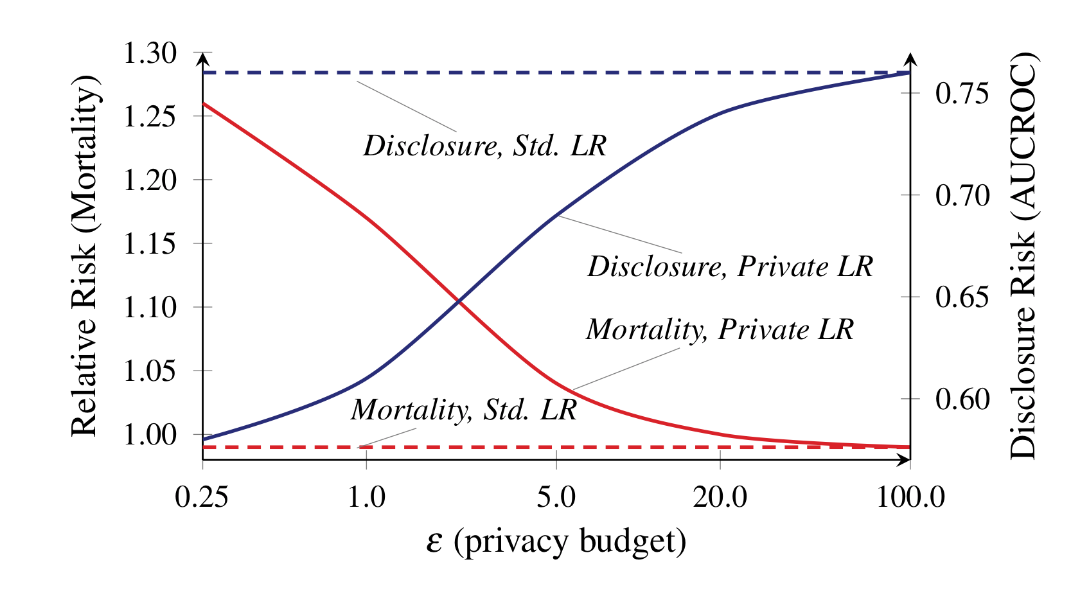
\includegraphics[width=\textwidth,height=\textheight,keepaspectratio]{warfarin.png}
\centering
\caption{Mortality and $\epsilon$}
\end{figure}
\end{center}

\paragraph{}
Using a dataset provided by the \textit{International Warfarin Pharmacogenetics Consortium} (IWPC), researchers at the University of Wisconsin constructed linear regression models designed to guide doctors in dosing. They then proceded to perform model inversion attacks to determine how much sensitive data these models would leak. These \textit{model inversion attack} would take the model and try to predict the presence or absence of specific genes in the individual genome.\cite{warfarin} Differential privacy would effectively combat these types of attacks, but at the risk of clinical efficacy. In fact, differential privacy became effective at $\epsilon \leq 1$, but the risk of either mortality or morbidity increased significantly, as can be seen in the figure above. Clearly the effectiveness of Differential Privacy is bounded in by the level of acceptable increase in mortality.

\section{Conclusion}

Genetic data has the capacity to both uniquely identify and reveal sensitive information about specific individuals and those related to them. The increase in the capabilities of the field bioinformatics has been met with increasing concern over genetic privacy. The malicious use of genetic data can lead to discrimination, exploitation, and identity theft. Gene data can also be stored indefinitely, and future techniques may tease out even stronger analytics than can be produced today. For these reasons, privacy in bioinformatics is a tremendously important topic in the field now and for the forseeable future.

\begin{thebibliography}{5}
  
\bibitem{naturegene} 
  https://www.nature.com/articles/35057062

\bibitem{nihfaq}
  https://www.genome.gov/19016904/faq-about-genetic-and-genomic-science/

\bibitem{vcf}
  http://www.internationalgenome.org/wiki/Analysis/vcf4.0
  
\bibitem{editdistance}
  http://repositorio.uchile.cl/bitstream\-/handle/2250/126168/Navarro\_Gonzalo\-\_Guided\_tour.pdf

\bibitem{warfarin}
  https://www.usenix.org/system/files/conference/usenixsecurity14/sec14-paper-fredrikson-privacy.pdf

\bibitem{natureped}
  https://www.nature.com/articles/nbt.4108
  
\end{thebibliography}
